\documentclass[12pt,a4paper]{article}
\usepackage[utf8]{inputenc}
\usepackage[brazilian]{babel}
\usepackage{amsmath}
\usepackage{float}
\usepackage{amsfonts}
\usepackage{amssymb}
\usepackage[T1]{fontenc}
\usepackage{graphicx}
\usepackage{physics}
\usepackage{siunitx}
\newcounter{prob}
\newcounter{subprob}
\renewcommand{\thesubprob}{\alph{subprob}}

\newcommand{\problem}{\setcounter{subprob}{0} \stepcounter{prob} \par \medskip \noindent \textbf{Problem~\theprob \ }}

\newcommand{\answer}{\par \medskip \noindent \textit{Resposta \ }}

\newcommand{\finalanswer}[1]{
	\begin{center} 
    	{\renewcommand{\arraystretch}{1.5}
		\renewcommand{\tabcolsep}{0.2cm} 
    	\begin{tabular}{|c|} 
    		\hline 
        	$ \displaystyle #1 $  \\ 
        	\hline 
    	\end{tabular}} 
   	\end{center}}

\newcommand{\subproblem}{\stepcounter{subprob} \par \smallskip \noindent \quad \textit{(\thesubprob) \ }}

\newcommand{\subanswer}{\par \smallskip \noindent \quad \textit{Resposta \ }}

\newcommand{\option}{\item[$\square$]}
\newcommand{\thisone}{\item[$\blacksquare$]}

\newenvironment{subitemize}{\begin{itemize}}{\end{itemize}}

%%%%%%%%%%%%%%%%%%%%%%%%%%%%%%%%%%%%%%%%%%%%%%%%%%%
\newcommand{\trans}{\mathsf{T}}
\newcommand{\hermit}{\mathsf{H}}
\newcommand{\mc}[1]{\ensuremath{\mathcal{#1}}}
\newcommand{\mbb}[1]{\ensuremath{\mathbb{#1}}}
\newcommand{\Natural}{\mathbb{N}}
\newcommand{\Integer}{\mathbb{Z}}
\newcommand{\Irrational}{\mathbb{I}}
\newcommand{\Rational}{\mathbb{Q}}
\newcommand{\Real}{\mathbb{R}}
\newcommand{\Complex}{\mathbb{C}}
\newcommand{\obs}[1]{\textcolor{red}{(#1)}}
%\newcommand{\iff}{\mbox{$\Longleftrightarrow$}}    % biimplication
% \newcommand{\and}{\wedge}
% \newcommand{\or}{\vee}
\newcommand*\diff{\mathop{}\!\mathrm{d}}
\newcommand*\Diff[1]{\mathop{}\!\mathrm{d^#1}}
\newcommand{\ensureoperation}{\negmedspace {}} % To ensure that a new line symbol is an operation instead of a sign
% \DeclarePairedDelimiter\abs{\lvert}{\rvert}%
% \DeclarePairedDelimiter\norm{\lVert}{\rVert}%

% Swap the definition of \abs* and \norm*, so that \abs
% and \norm resizes the size of the brackets, and the 
% starred version does not.
% Usage example
% \abs{x} \norm{x}
% \abs*{x} \norm*{x}
\makeatletter
\let\oldabs\abs
\def\abs{\@ifstar{\oldabs}{\oldabs*}}
%
\let\oldnorm\norm
\def\norm{\@ifstar{\oldnorm}{\oldnorm*}}
\makeatother

%%%%%%%%%%%%%%%%%%%%%%%%%%%%%%%%%%%%%%%%%%%%%%%%%%%







\author{Aluno - Código do Aluno}
\title{Lista de Exercícios - Código da Disciplina}
\date{}
\begin{document}

%%--CABEÇALHO--%%
	\begin{center}
    {\huge Exercise list n1\par}
    {\LARGE Multlinear transformations and Multlinear rank \par}
    {\Large Engenharia de Telecomunicações \par}
    {\Large Professor Henrique Goulart \par}
    \end{center}

\problem \label{probone}

Let us define \(\mathcal{X} \in \Complex^{I_1 \times I_2 \times \cdots \times I_N}\) and \(\mathbf{U}^{(n)} \in \Complex^{J_n\times I_n}\), the n-mode product is defined as
\begin{align}
    \label{eq:n-mode-prod}
    \mathcal{Y} & = \mathcal{X}\times_n \mathbf{U}^{(n)}
\end{align}

where \(\mathcal{Y} \in \Complex^{I_1 \times \cdots I_{n-1} \times J_{n} \times I_{n+1} \times I_N}\) is a tensor obtained multiplying each n-mode fiber of \(\mathcal{X}\) by $\mathbf{U}^{(n)}$. The element-wise operation is given by
\begin{align}
    y_{i_1, \cdots, i_{n-1}, j_{n}, i_{n+1}, i_N} = \sum_{i_n}^{I_n} x_{i_1, i_2, \cdots, i_N} u_{j_n, i_n}
\end{align}

Hence,
\begin{align}
    \mathcal{Z} & = T\left\{\mathcal{X}\right\} \\
    & = \mathcal{X}\times_1 \mathbf{U}^{(n)}\times_2 \mathbf{U}^{(2)} \cdots \times_N \mathbf{U}^{(N)}
\end{align}
gives a multlinear transformation (denoted by $T\left\{\right\}$) , where $\mathcal{Z} \in \Complex^{J_1 \times J_2 \times \cdots \times J_N}$. The multilinear transformation can be interpreted in two equivalent ways: In the first one, it represents the mathematical operation that leads \(\mathcal{X}\) to \(\mathcal{Z}\), that is, the values of new tensor stem from changing of the values of \(\mathcal{X}\). In the second one, \(\mathcal{X}\) is thought as a fixed element in a multidimensional space, and $T\left\{\right\}$ changes the vector basis of that space. In this case, the values of new tensor stem from changing the vector basis used to represent \(\mathcal{X}\). In the particular case where \(J_n = I_n\), we have that \(\mathcal{Z} \in \Complex^{I_1 \times I_2 \times \cdots \times I_N}\) and each vector basis remains with the same dimensionality.

It is important to notice that there is a \emph{isomorphism} between the mapping from the Eq. \eqref{eq:n-mode-prod} and
\begin{align}
    \left[\mathcal{Z}\right]_{(n)} = \mathbf{U}^{(n)} \left[\mathcal{X}\right]_{(n)},
\end{align}
where \(\left[\mathcal{X}\right]_{(n)}\) is the n-mode unfolding of the tensor \(\mathcal{X}\). The n-rank of \(\mathcal{Z}\), \(R_n = rank\left(\left[\mathcal{Z}\right]_{(n)}\right)\), is given by
\begin{align}
    \label{eq:n-rank}
    R_n &= rank\left(\left[\mathcal{X}\times_1 \mathbf{U}^{(n)}\times_2 \mathbf{U}^{(2)} \cdots \times_N \mathbf{U}^{(N)}\right]_{(n)}\right) \\
    &= rank\left(\mathbf{U}^{(n)} \left[\mathcal{X}\right]_{(n)} \left(\mathbf{U}^{(N)} \otimes \cdots \otimes \mathbf{U}^{(n+1)} \otimes \mathbf{U}^{(n-1)} \otimes \cdots \mathbf{U}^{(1)}\right)^\trans \right)\\
    &= rank\left(\mathbf{U}^{(n)} \left[\mathcal{X}\right]_{(n)} \mathbf{V} \right),
\end{align}
where $\mathbf{V} = \left(\mathbf{U}^{(N)} \otimes \cdots \otimes \mathbf{U}^{(n+1)} \otimes \mathbf{U}^{(n-1)} \otimes \cdots \mathbf{U}^{(1)}\right)^\trans$, being \(\otimes\) the Kronecker product. For the constraint where \(\left\{\mathbf{U}^{(n)}\right\}\) is a set of non-singular matrices, we have that
\begin{align}
    rank\left(\mathbf{U}^{(n)}\right)&= I_n \\
    rank\left(\left[\mathcal{X}\right]_{(n)}\right)&= r_{x,n} \\
    rank\left(\mathbf{V}\right)&={I_n}^{N-1}
\end{align}
and
\begin{align}
    R_n = min\left(I_n, r_{x,n}\right)
\end{align}
The n-rank of \(\mathcal{Z}\) is equal to \(\mathcal{X}\) as $r_{x,n}$ does not depends on the multlinear transformation. Hence, the multilinear rank, given by \(rank\left(\mathcal{X}\right)-\left(R_1,R2,\cdots, R_N\right)\) is property of the tensor \(\mathcal{X}\).



%*************************************************
\problem O sinal de tempo contínuo \(x_c(t)\) com a transformada de Fourier \(X_c(j\Omega)\) mostrada na Figura \ref{fig:1} passa pelo sistema mostrado na Figura \ref{fig:2}. Determine o intervalo de valores de T para o qual \(x_r(t)\) = \(x_c(t)\)

\begin{figure}[h!]
    \centering
    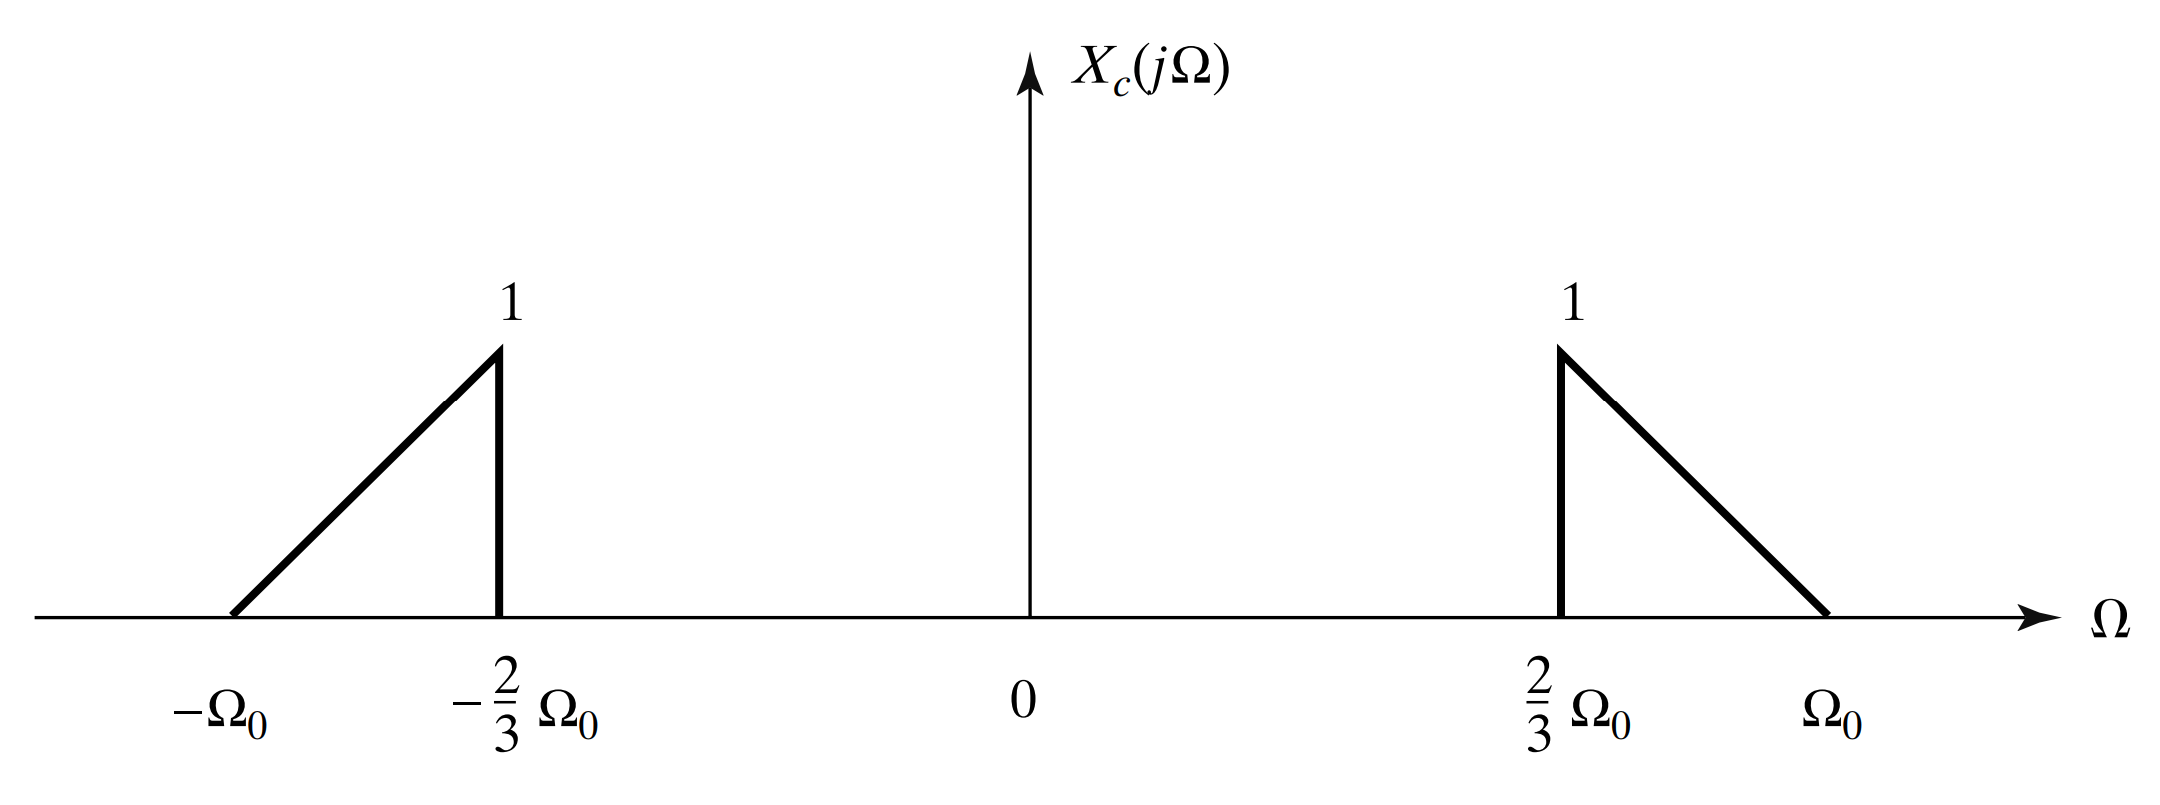
\includegraphics[scale=0.5]{./figs/prob1.png}
    \caption{Figura para solução do Problem 1.}
    \label{fig:1}
\end{figure}

\begin{figure}[H]
    \centering
    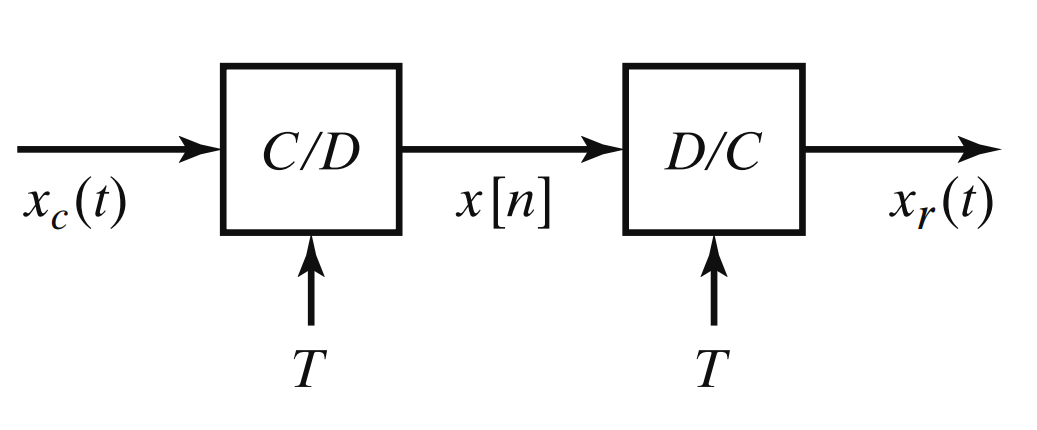
\includegraphics[scale=0.5]{./figs/prob2.png}
    \caption{Figura para solução do Problem 1.}
    \label{fig:2}
\end{figure}

\answer
%============================================
\problem Considere a representação do processo de amostragem seguido pela reconstrução mostrada na Figura \ref{fig:22}.

\begin{figure}[h!]
    \centering
    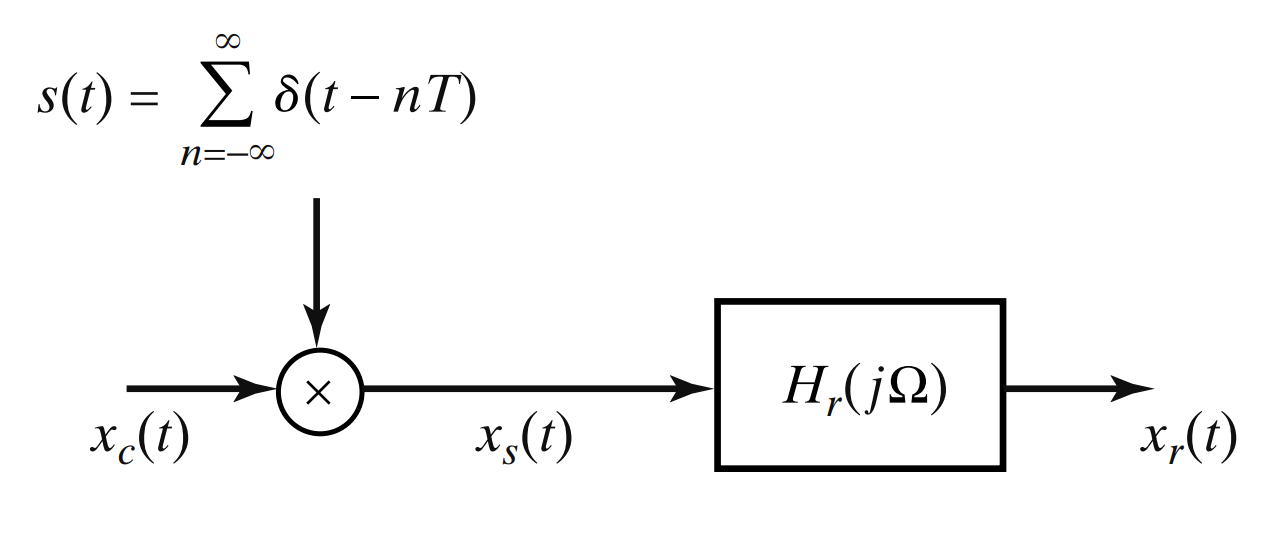
\includegraphics[scale=0.5]{./figs/prob22.png}
    \caption{Figura para solução do Problem 2.}
    \label{fig:22}
\end{figure}

Assuma que o sinal de entrada seja
\[\begin{array}{lr}
    x_c(t) = 2 \cos(100\pi t - \pi /4) + \cos(300\pi t + \pi /3) & -\infty < t < \infty
\end{array}\]

A resposta em frequência do filtro de reconstrução é
\[H_r(j \Omega) = \left\{ \begin{array}{lr}
    T, & \left|\Omega\right| \leq \pi/T \\
    0, & \left|\Omega\right| > \pi/T
\end{array} \right.\]

\subproblem Determine a transformada de Fourier de tempo contínuo \(X_c(j\Omega)\) e a esboce como uma função de \(\Omega\).
\subproblem Suponha que \(f_s = 1/T = 500\) amostras/s e esboce a transformada de Fourier \(X_s(j\Omega)\) em função de \(\Omega\) para \(-2\pi/T \leq \Omega \leq 2\pi/T\). Qual é a saída \(x_r(t)\) nesse caso? (Você deverá ser capaz de dar uma expressão exata para \(x_r(t)\).)

\answer
%=================================================
\problem Desenhe o diagrama de fluxo de sinais para a implementação na forma direta I do sistema LIT com função de sistema

\begin{equation}
    H(z) = \frac{1- \frac{1}{2}z^{-2}}{1- \frac{1}{4}z^{-1} - \frac{1}{8}z^{-2}}
\end{equation}

\answer
%========================================================
\problem Determine a resposta ao impulso \(h\left[n\right]\) para um filtro FIR de fase linear com comprimento \(M=4\), cuja a resposta em frequência satisfaça
\[
\begin{array}{lr}
    H_r \left(0\right), & H_r \left(\frac{\pi}{2}\right) = \frac{1}{2}.
\end{array}
\]

\answer
%=========================================================
\problem Use a transformação bilinear para converter o filtro analógico
\[H(s) = \frac{s+1}{(s+0,1)}^2+9\]
para um filtro digital IIR. Selecione \(T=0,1\).

\problem Repita a questão anterior, mas desta vez use o m\'etodo da invariância ao impulso. Por fim, compare a localização dos zeros com a localização dos zeros obtidas na questão anterior.


\end{document}